\section{In Vitro Experiments}

\begin{figure}[t]
    \centering
    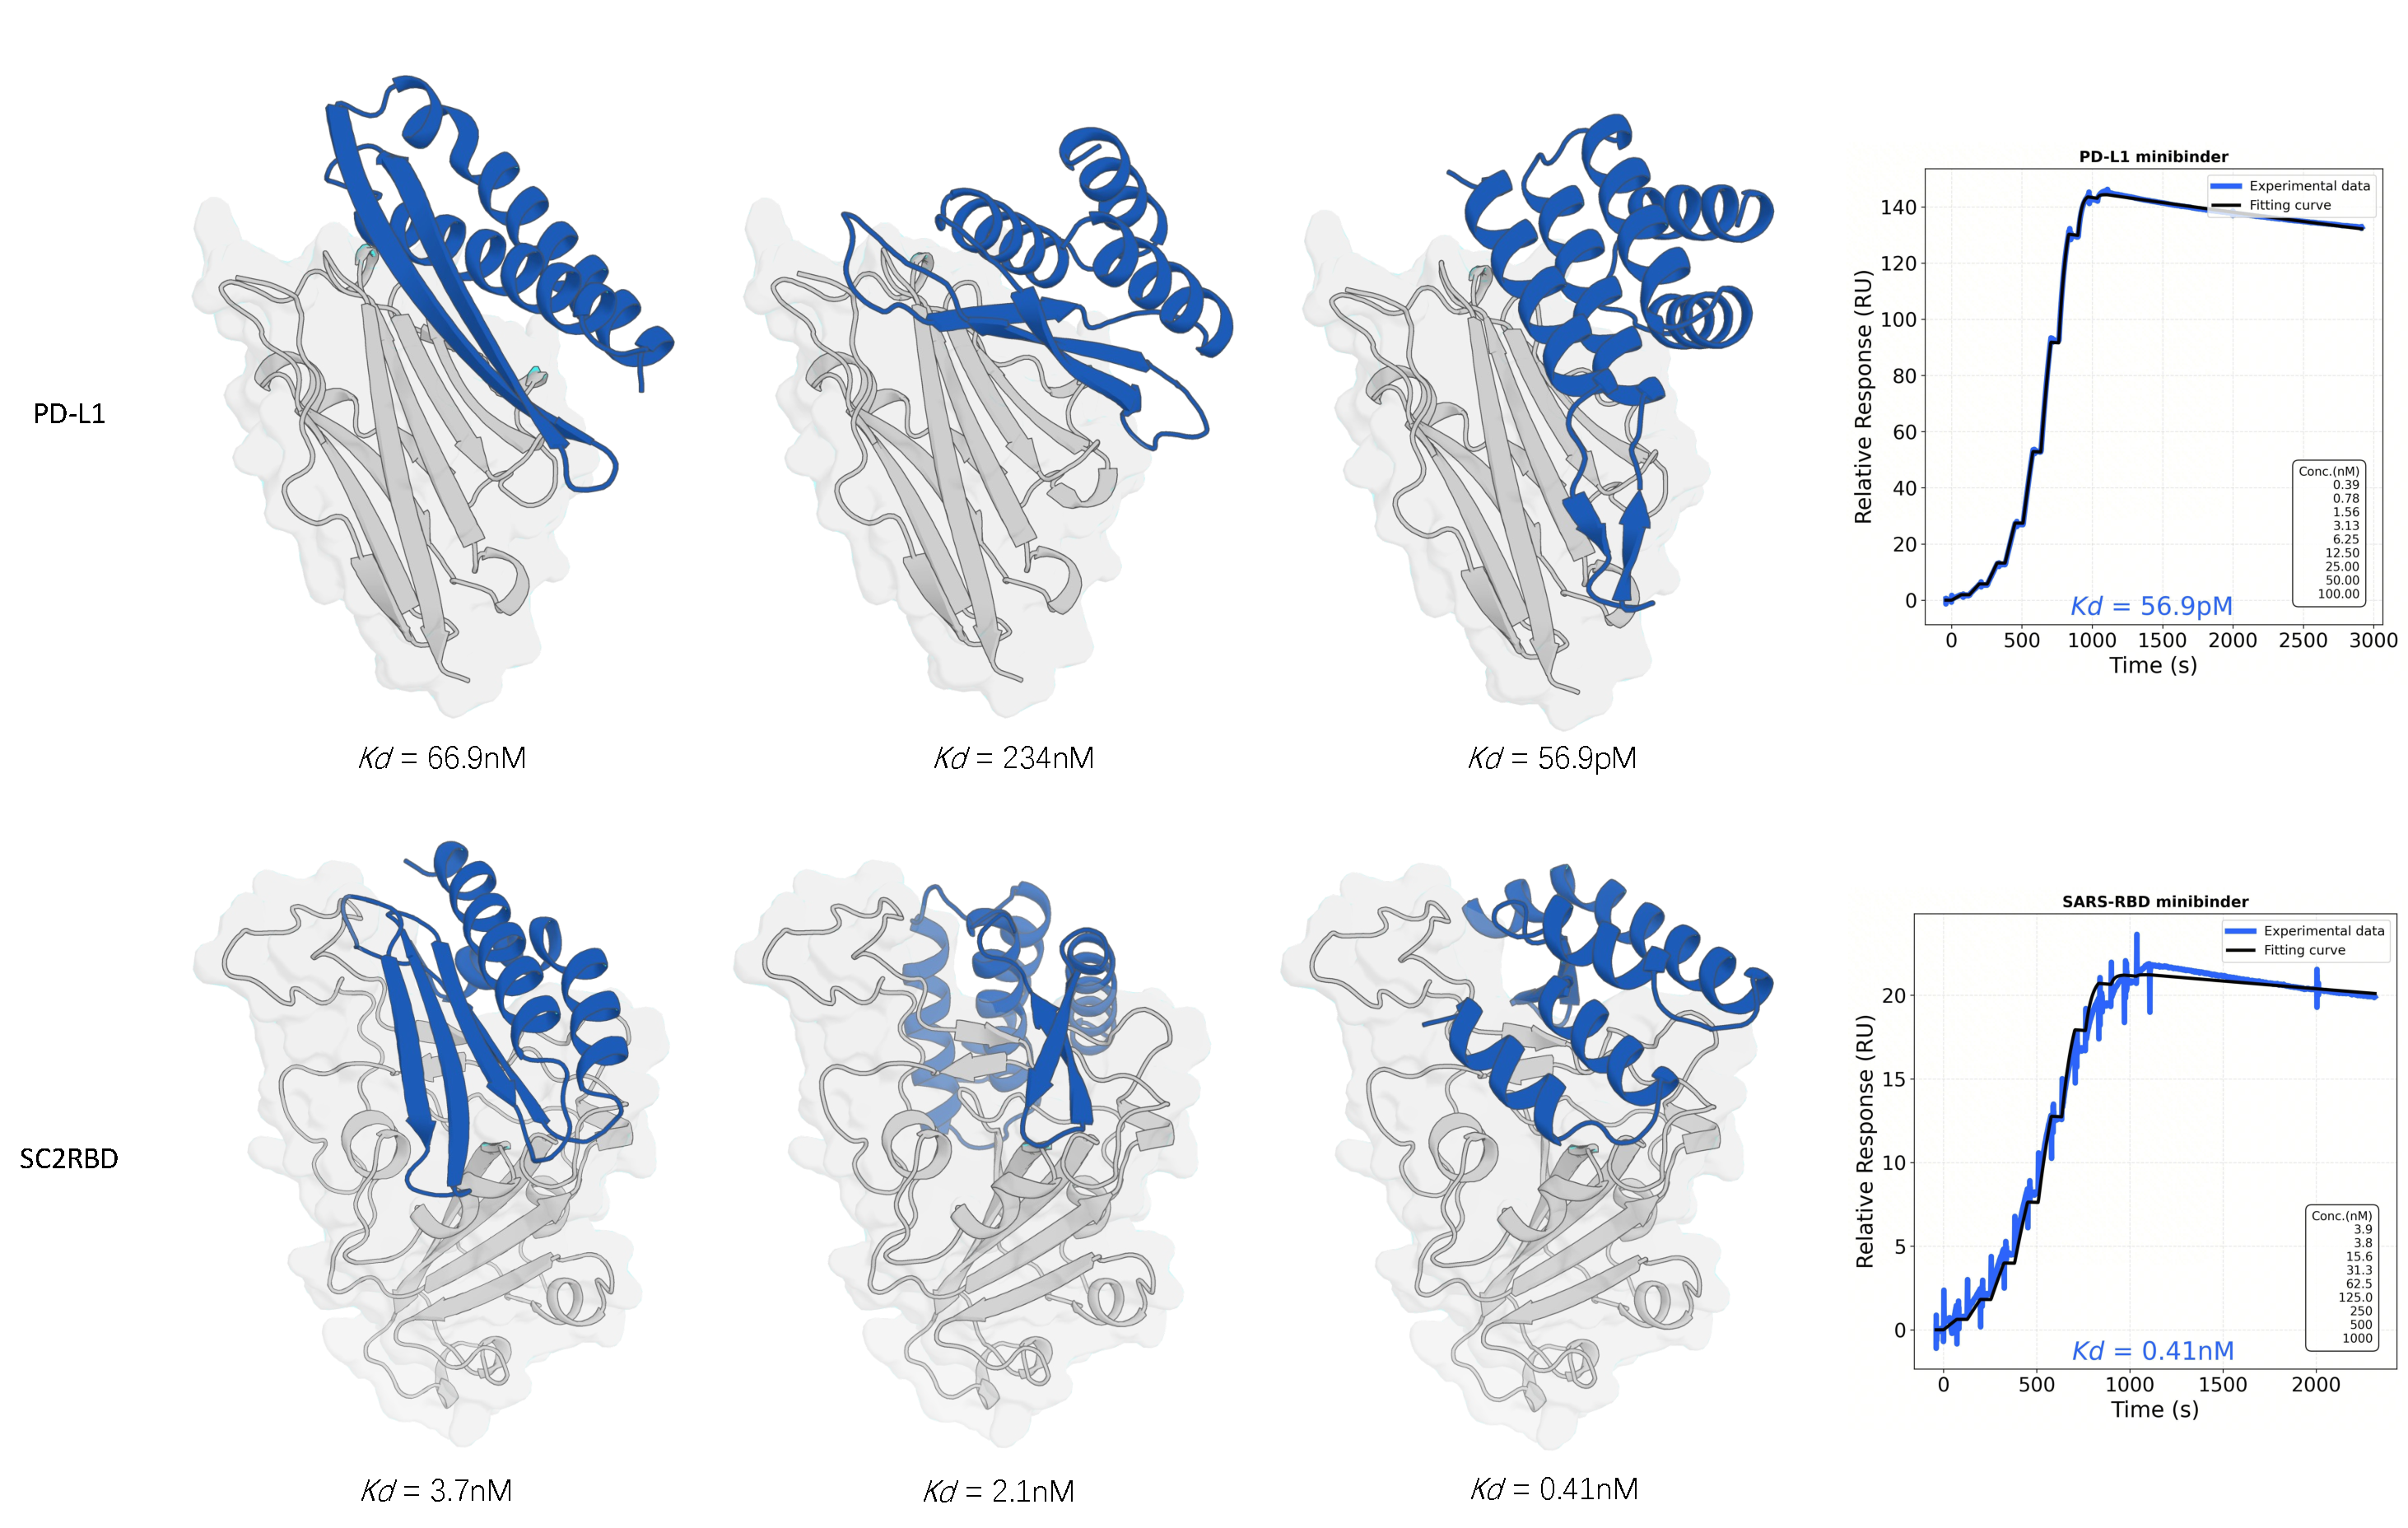
\includegraphics[width=0.95\linewidth]{figures/wetlab_res.pdf}
    \caption{Wet-lab validation of SeedProteo-designed binders. For each target (PD-L1, top; SC2RBD, bottom), three representative binding complex structures are shown alongside the SPR sensorgram of the highest-affinity binder.}
    \label{fig:wetlab_res}
\end{figure}

To validate the practical utility of SeedProteo beyond in-silico metrics, we conducted wet-lab experiments on two therapeutically relevant protein targets: the SARS-CoV-2 receptor-binding domain (SC2RBD) \cite{cao2020novo} and Programmed Death-Ligand 1 (PD-L1) \cite{yang2025design}. These targets were selected due to their high clinical relevance---SC2RBD is a primary target for COVID-19 therapeutic antibody development, while PD-L1 is a critical immune checkpoint widely pursued in cancer immunotherapy---as well as their structural diversity, which allows us to assess the generalizability of our model across distinct binding interfaces.

For each target, we generated several thousand minibinders using SeedProteo. The structures passing the in-silico criteria were further clustered using Foldseek to ensure structural diversity, from which 10 representative minibinders were selected per target for experimental characterization. The selected minibinders were recombinantly expressed in \textit{E.~coli} with an N-terminal His-SUMO tag and purified via Ni-NTA affinity chromatography followed by size-exclusion chromatography (detailed protocols in Appendix~\ref{app:protein_production}). Binding properties were characterized using surface plasmon resonance (SPR) on a Biacore~8K+ instrument, where candidates were first screened at two concentrations and then subjected to kinetic affinity measurements using either single-cycle or multi-cycle protocols (Appendix~\ref{app:spr}). Protein expression and SPR assays for all designed candidates were performed by WuXi AppTec (China).

As shown in Figure~\ref{fig:wetlab_res}, SeedProteo achieved hit rates of 70\%--80\% across both targets, with the best binders reaching picomolar affinity for PD-L1 and sub-nanomolar affinity for SC2RBD. These results demonstrate that our in-silico design pipeline reliably produces binders with strong experimental binding, bridging the gap between computational prediction and wet-lab validation.
